\documentclass[simplex.tex]{subfiles}
% NO NEED TO INPUT PREAMBLES HERE
% packages are inherited; you can compile this on its own
\begin{document}
\subsection{Reduced Dimension Clustering}
%
%We develop a new statistical method, named ``automatic repulsive
%clustering'' (ARC, to handle the clustering problem when the
%dimensionality outgrows the number of the data points. The standard
%dimension reduction tool such as principle component analysis (PCA) is
%not optimal for finding the subspace best suitable for clustering.
%Therefore, we seek the method to do dimension reduction and clustering
%at the same time: we develop a regularization to encourage good
%separation of the clusters, forcing the subspace to an angle so that
%each point can belong to a cluster completely. The plots below shows the
%different performances in clustering a equally proportioned 3
%components: the subspace found by PCA leads to incorrect clustering of
%the data, due to the orientation of the space; whereas ARC successfully
%identifies the ideal clustering direction in one dimensional space,
%hence generating satisfactory clustering result.
%
%
%\begin{figure}[h!]
%\begin{cframed}
%\centering
%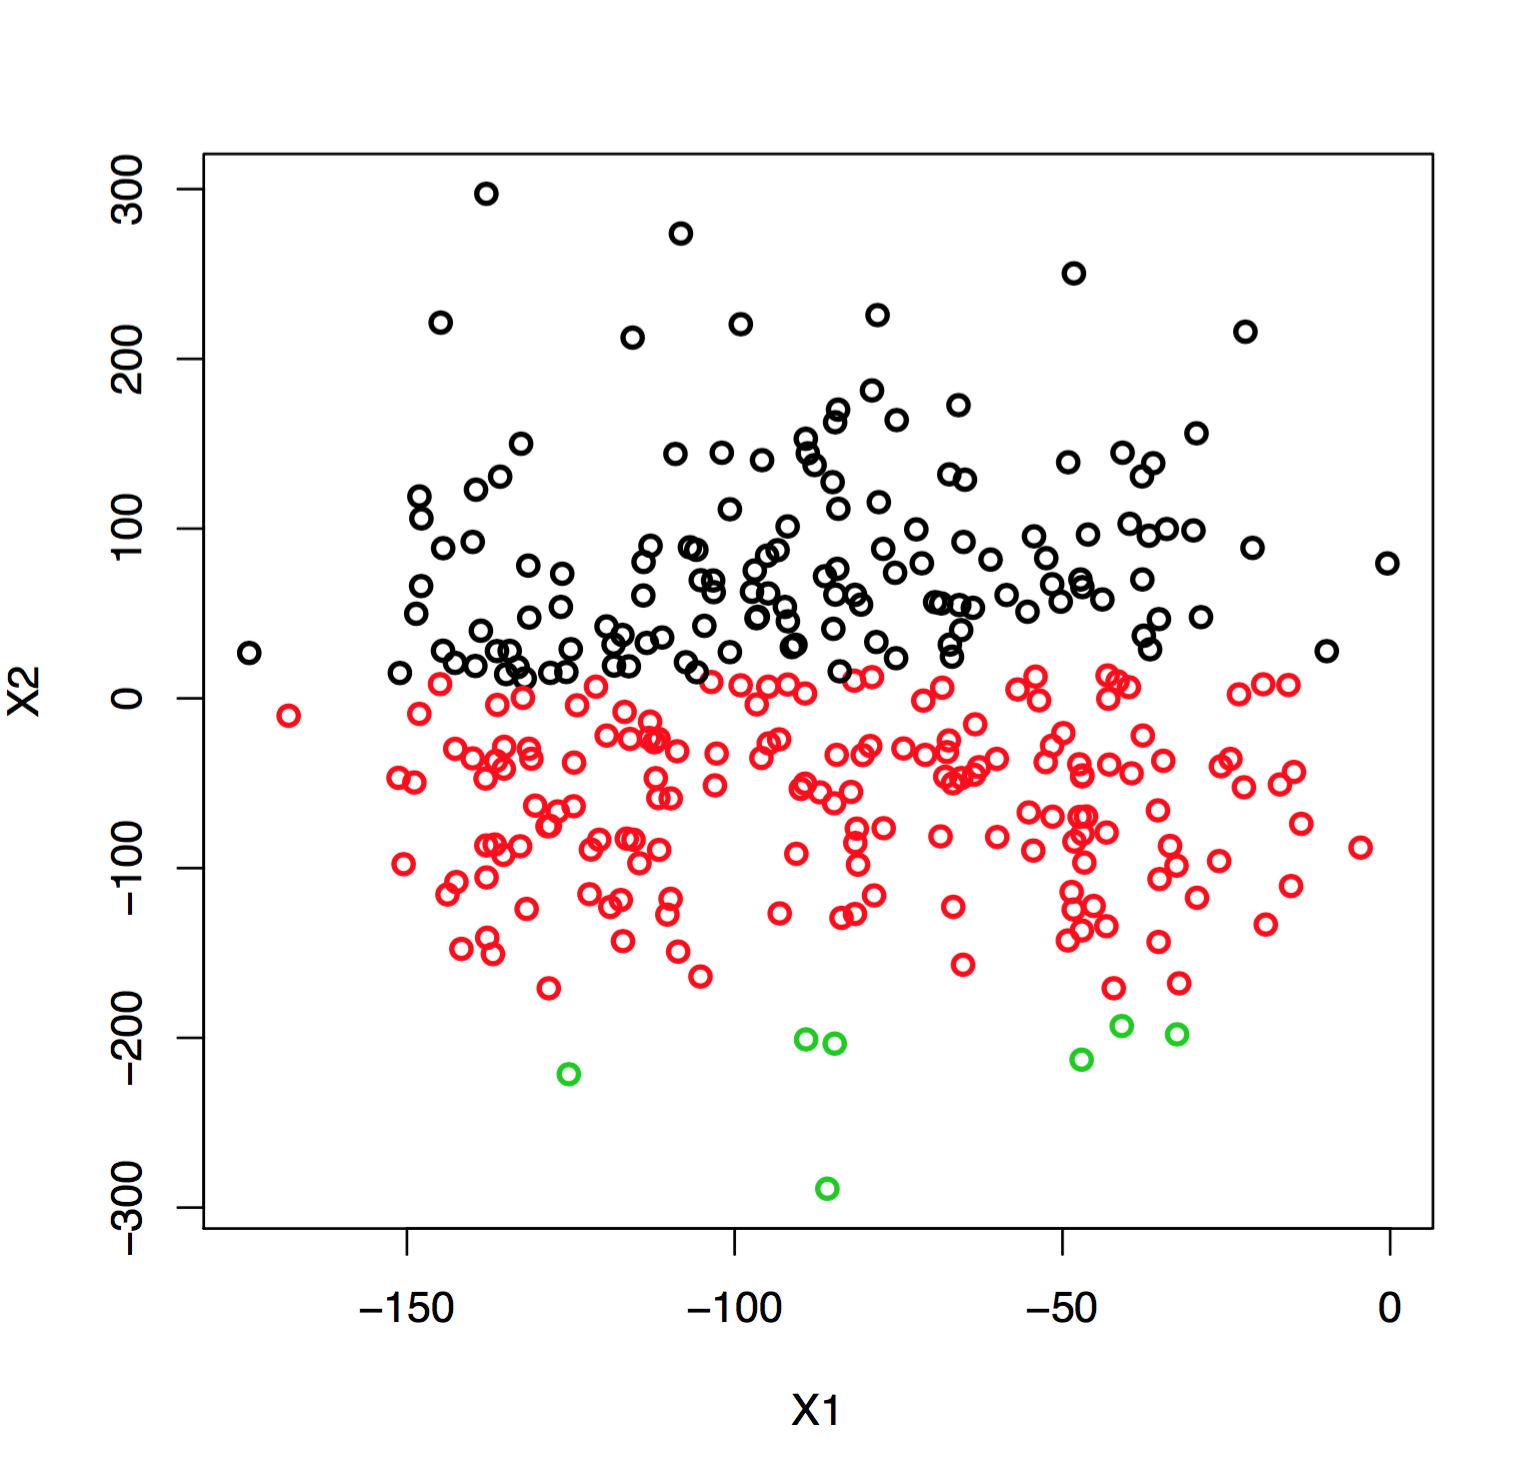
\includegraphics[width=0.45\textwidth]{../../figs/pcaBased.png}
%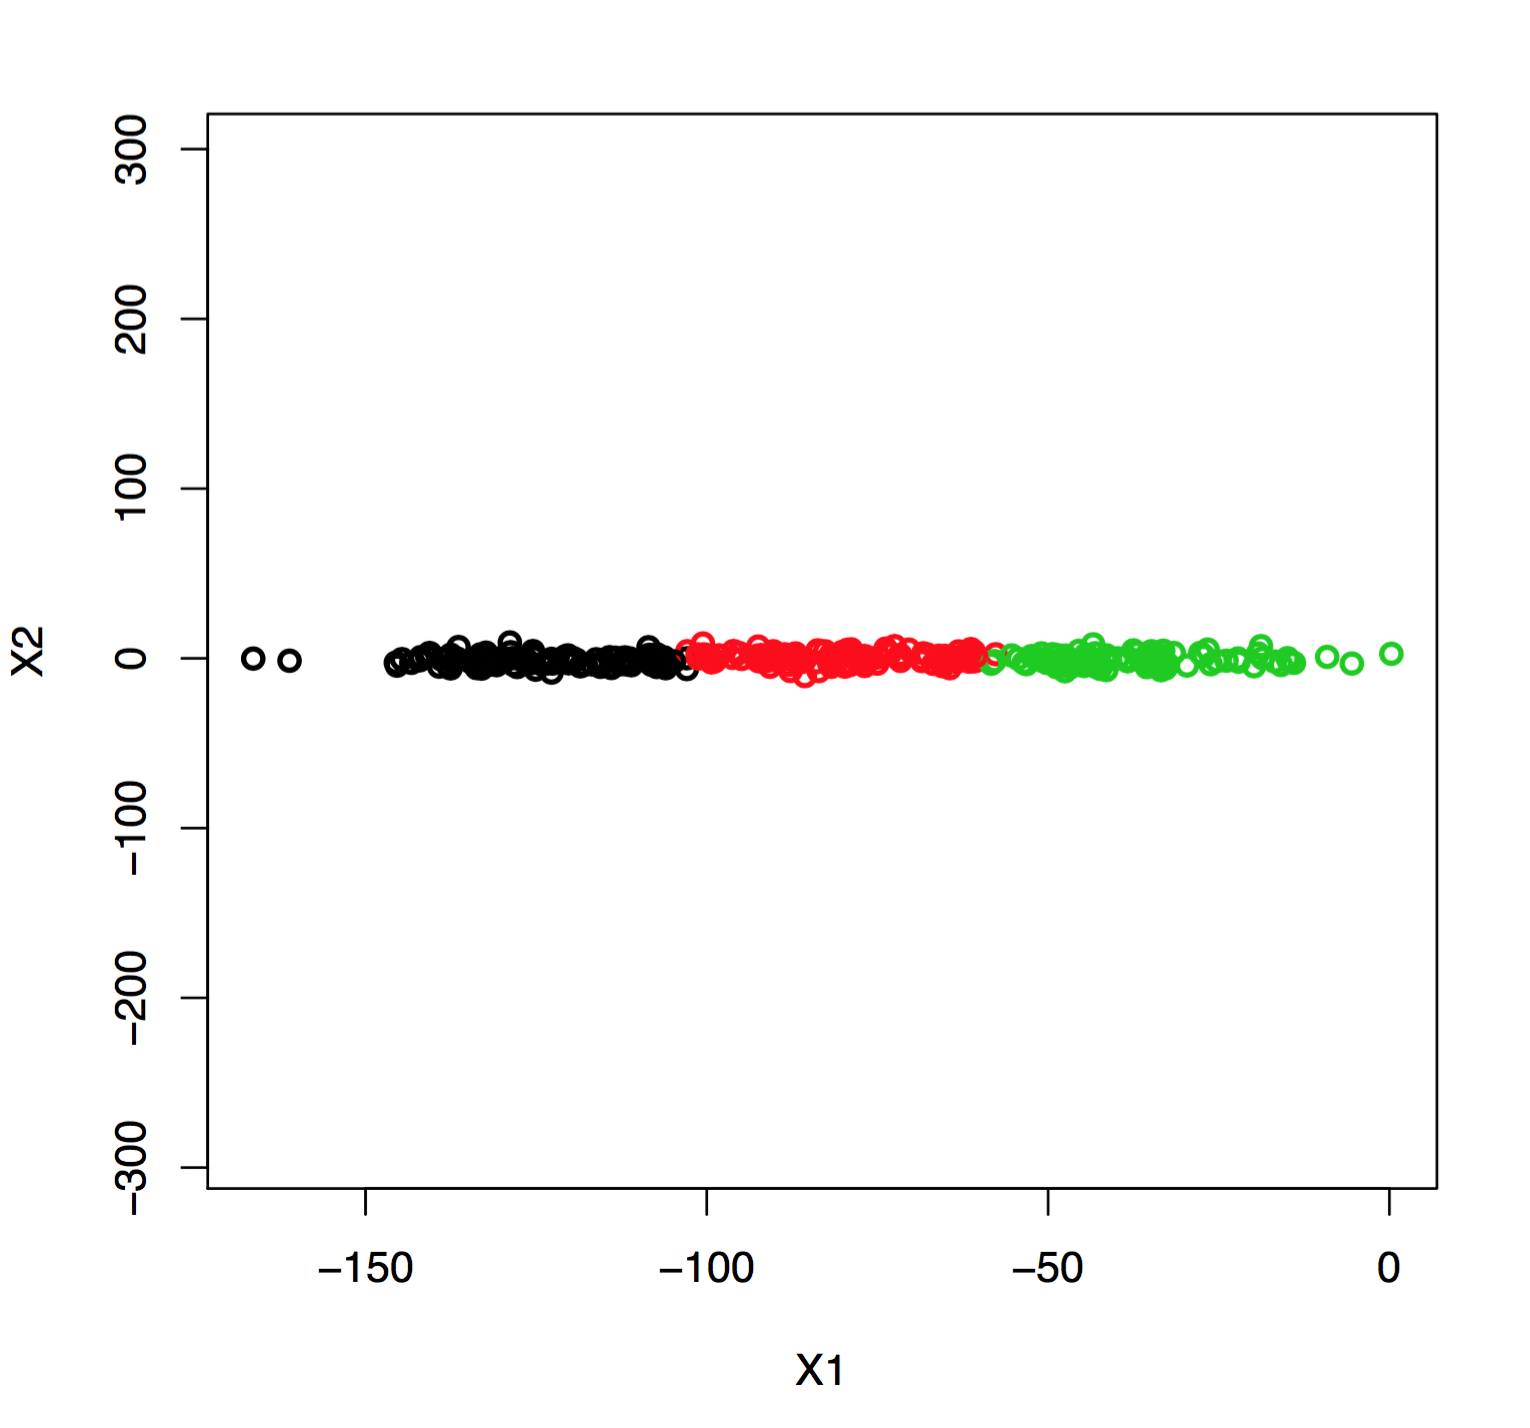
\includegraphics[width=0.45\textwidth]{../../figs/ARC.png}
%\caption{PCA (left) versus Reduced Dimension Clustering (right).}
%\label{fig:arc}
%\end{cframed}
%\end{figure}
%
%
\end{document}
